\section{Background on \bc and Its Network Traffic}\label{sec:back}


\bc is the most popular cryptocurrency. It uses  a decentralized, peer-to-peer architecture~\cite{nakamoto2008bitcoin}, where each peer (e.g., client) is identified by her unique public key.  
	\bc clients exchange money through \bc transactions, which are  broadcasted on \bc's p2p network. 

	To prevent double spending and similar violations, \bc uses a public ledger called the \emph{blockchain} to store all \bc transactions. The blockchain is a chain of \emph{blocks}, where  each block contains a set of transactions and a \textit{proof-of-work}. A proof-of-work is a piece of data which is time-consuming and costly to generate. However, verifying the proof-of-work is easy. Each block is valid if and only if all of its transactions and its proof-of-work are valid. A verified block is broadcast on the network to update all peers' local ledgers. 
\begin{comment}	
\paragraphb{\bc's P2P Network.}
	\bc nodes form a full-mesh P2P network, and they connect to each other over unencrypted TCP connections. 
	Each node can connect to up to 125 peers, where up to 8 of them are  outgoing connections and the rest are incoming connections. A node stays connected to a neighbor until they restart or drop, in which case the node tries to replace them~\cite{Bitcoinnetworkoverview}. 
	%Since connection is without authentication, peers just keep a list of their connection IP addresses.
	Blocks and transactions are propagated by gossip. To avoid DoS attacks, peers only forward valid blocks and transactions; invalid blocks are discarded. 
	\end{comment}
%Bitcoin peers can be separated into two types: routable and non-routable. The former are capable of accepting incoming connections, and the latter are not, for example because they are behind a NAT or firewall.% However, it is worth mentioning that the official {\tt Bitcoind} software does not precisely split its functionality among routable and non-routable peers. 

\paragraphb{\bc Protocol Messages.}
	 \bc communications involve various protocol messages that are created by \bc peers. 
	 We divide \bc protocol messages into two classes: \emph{synchronization messages},  which are used for  propagating user addresses and transactions in the \bc network, and \emph{block-related messages}.%, which are responsible for disseminating \bc blocks. We introduce  major \bc messages in  Table~\ref{tab:bc-proto-list}.
	
%\section{Characterizing \bc Traffic}\label{sec:char}
\subsection{Synchronization Messages}
These messages are aimed at keeping \bc peers synchronized with the rest of the \bc network. %These messages are as following: \textbf{addr}, \textbf{inventory(inv)},\textbf{getdata}, and \textbf{tx}.

\code{\textbf{addr:}}Each peer advertises the information and IP addresses of other peers via \code{\textbf{addr}} message in the network. %\code{addr} message contains count and list of other peers IP addresses. Each IP address is accompanied by a timestamp showing its freshness. When a peer receives a list of addresses from other peers, it has a choice to forward any number of them. The peer chooses the sending addresses based on the following criteria: 1)~The number of IP addresses in the received message should not be greater than 10,and 2)~The timestamps should not be older than 10 minutes. This mechanism is applied for helping in peer discovery. 

\code{\textbf{inventory(inv):}} Peers send \code{inv} to advertise their knowledge about the known objects, like transactions and blocks.% Each \code{inv} message consist of number of inventory entries and the inventory vectors itself.% It can be received unsolicited, or in reply to \code{getblocks}.
%Inventory vectors  are used for notifying other nodes about objects they have or data which is being requested. Inventory vectors consist of the type of objects and the hash of the object. 

\code{\textbf{getdata:}} A peer sends \code{getdata} message in response to the \code{inv} to retrieve information about the content of an object, which can be a block or a transaction. 

\code{\textbf{tx}:} This message describes a transaction in response to a \code{getdata} message.% Each transaction is stored in a memory pool. If a received transaction is already in the pool, or it is included in one of the blocks in the main block-chain, it get discarded. 

% then the receiving peer runs several checks on the transaction's advertisement. If the checks passed, then the receiving peer asks for the transactions.

\subsection{Block-Related Messages} Such messages are used to exchange \bc blocks among the peers. 
The current \bc network is supporting two ways of propagating blocks, full block and compact block
propagation. %Figure~\ref{fig:protocol-flow} demonstrates the flow of message communication in these
%two ways.

\begin{comment}
  \begin{figure}[h]
\centering
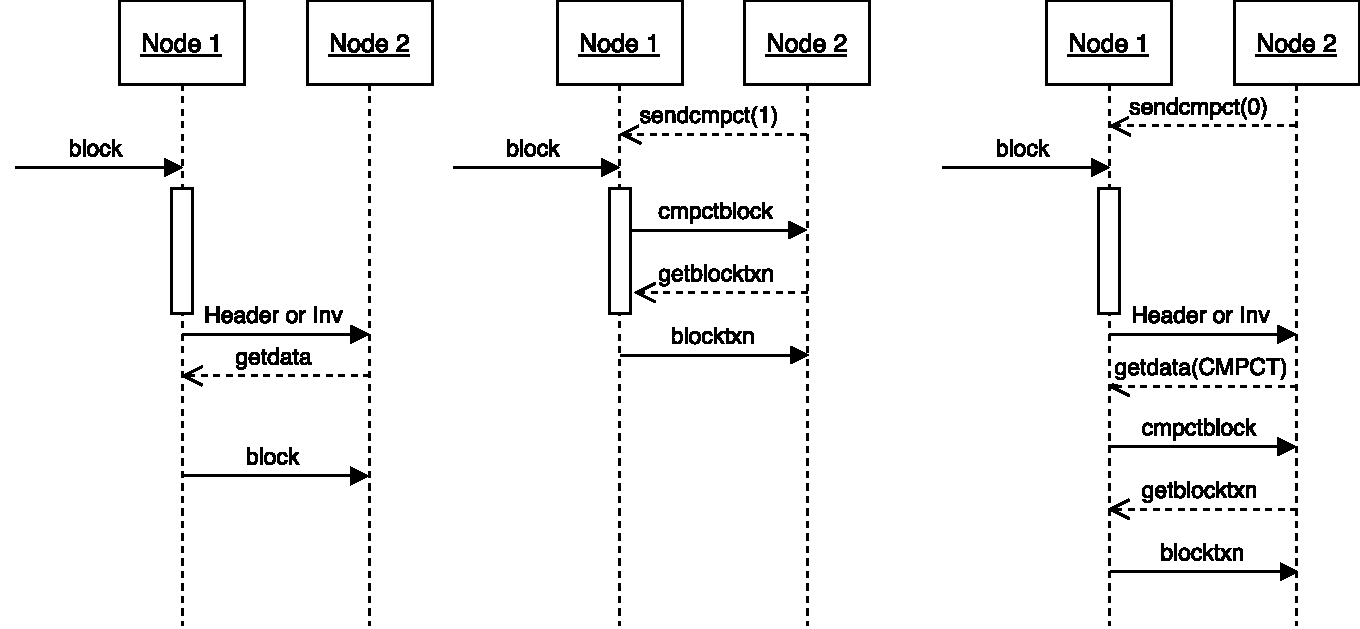
\includegraphics[scale=0.45]{image/btc-protocol-flow.pdf}
\caption{Different relaying modes in  Bitcoin}
\label{fig:protocol-flow}
\end{figure}
\end{comment}

\paragraphe{Full Block Propagation:} The sender node first validate the block completely, then it advertise the possession of block by \code{inv} message. The receiving peer which doesn't have the block, asks for it by sending \code{getdata} message. Finally, the sender node send the block via \code{block} message. Sending full block in the network is wasting network bandwidth since we are re-sending all of the transaction and nodes have some of transaction in their memory pool. The messages transmitted in this mode is: 

\code{\textbf{block:}} It consist of block version information, previous block hash, merkle root of a Merkle tree collection which is a hash of all transactions related to this block. Sending  the new block forwarded through all the network.

%\amir{the two parts are uneven regarding how much you discuss}
\paragraphe{Compact Block Propagation:}
From the middle of 2016 in \code{0.13.0} version, Bitcoin protocol start to forward blocks as compact blocks which means instead of forwarding full blocks in network, only a sketch of block is sent. The sketch include 80-byte block's header, the short transactions IDs used for matching already-available transactions and select of transactions which sending peer expect that a receiving peer may be missing.% After receiving the compact block, the receiving peer tries to reconstruct the block at its end, from the already received transactions and the one in compact block. In this way the waste of sending each transaction twice is reduced. The advantage of compact block relaying is reducing the spikes in the bandwidth and  also reduce propagation delay. The messages transmitted in this mode are: 

\code{\textbf{sendcmpct:}} This message informs the receiving peer about the mode of communication the sending peer has chosen (low or high bandwidth). %If the first byte of the message is set to 1 the sender is indicating that it wants to receive blocks as soon as possible and it is working in the high-bandwidth mode. If the first byte of the message is set 0 the sender is saying that it wants to minimize bandwidth usage as much as possible and it is working in the low-bandwidth mode.

\code{\textbf{cmpctblock}:} This message introduced in the compact block relaying and is presenting a sketch of block.

\code{\textbf{getblocktxn}:} This message is introduced in compact block relaying and is used to request for the transactions that are missed by sending a list of their indexes. 

\code{\textbf{blocktxn}:} This message is introduced in compact-block relaying and is used to provide some of the transactions in a block, as requested.

\begin{comment}
Compact block relaying works in high and low bandwidth settings. In high bandwidth the receiving peer doesn't oblige the sending peers to ask for permission first. So, multiple peers can send the compact block to receiving node. Then at last the sender node sends the missing transactions by \code{blocktxn} message. It is worth mentioning \bc works in high bandwidth mode with up to 3 peers. 
However, in low bandwidth mode, since bandwidth is its bottleneck, the receiving node oblige other nodes to ask for permission first. So, the sender first advertise the block possession by \code{inv} message. Then, the receiving node asks for the compact block by \code{getdata} and the sender will send the compact block by \code{cmpctblock} message. At last, if there is any missing transaction, the receiving node will ask for it by \code{getblocktxn} and the sender will send those transactions via \code{blocktxn}. 
\end{comment}
\begin{comment}


\begin{table*}[!h]
\caption{The list of Bitcoin communication messages}\label{tab:bc-proto-list}
\centering
\begin{tabular}{| c | l |} \hline
Message & Description \\ \hline
\code{version}
& \shortstack{Advertise the node's version. No further communication is possible until \\both peers have exchanged their version.}  \\ \hline
\code{verack}
& Reply to the \code{version} message. \\ \hline
\code{addr}
& Send information about the known nodes of the network. \\ \hline
\code{inv}
& \shortstack{Sent to advertise the knowledge of the peer about the known objects. It can be received unsolicited, \\or in reply to \code{getblocks}.} \\ \hline
\code{getdata}
& Sent in response to the \code{inv} message to retrieve information about the content of an object. \\ \hline
\code{notfound} & If the receiver of \code{getdata} cannot return the requested information, it respond with \code{notfound} \\ \hline
\code{getblocks} & It return an \code{inv} message with the list of block after the specified block in \code{getblocks} request \\ \hline
\code{getheaders} & It return a \code{headers} message with the list of block after the specified block in \code{getblocks} request \\ \hline
\code{tx} 
& Sent to describes a Bitcoin transaction in response to a 
\code{getdata} message. \\  \hline
\code{block} &  \code{block} message is sent in response to a \code{getdata} message \\ \hline
\code{headers} &  Return a list of block headers, in respond to \code{getheaders} \\ \hline
\code{getaddr} & A node sends \code{getaddr} to ask about the known peer  from other peers  \\ \hline
\code{mempool} & It asks about the transaction in mempool of other peers \\ \hline
\code{ping}
& Show the TCP/IP connection is still valid. \\ \hline
\code{pong}
& Response to \code{ping} message. \\ \hline
\code{reject} & It show a message has been rejected \\ \hline
\code{sendheaders} & let other peers to send headers without \code{inv} message \\ \hline
\code{sendcmpct} &  let other peers to send compact blocks   \\ \hline
\code{cmpctblock} & it used in stead of \code{block}, to send cmpctblock \\ \hline
\code{getblocktxn} & it indicate missing block in compact block transaction \\ \hline
\code{blocktxn} & To send missing block in compact block transaction \\ \hline
\end{tabular}
\label{table:msg_description}
\end{table*}
\end{comment}


\begin{comment}
\section{Distribution of Packet Sizes over Tor}\label{sec:bcshape}

Figure~\ref{fig:tor_reg_traffic_pkt_size_upstream}-\ref{fig:tor_fullblock_pkt_size_downstream} shows the upstream and downstream packet distribution of HTTP and \bc traffic behind Tor.
\begin{figure}[t]
\begin{subfigure}{0.48\linewidth}
\centering
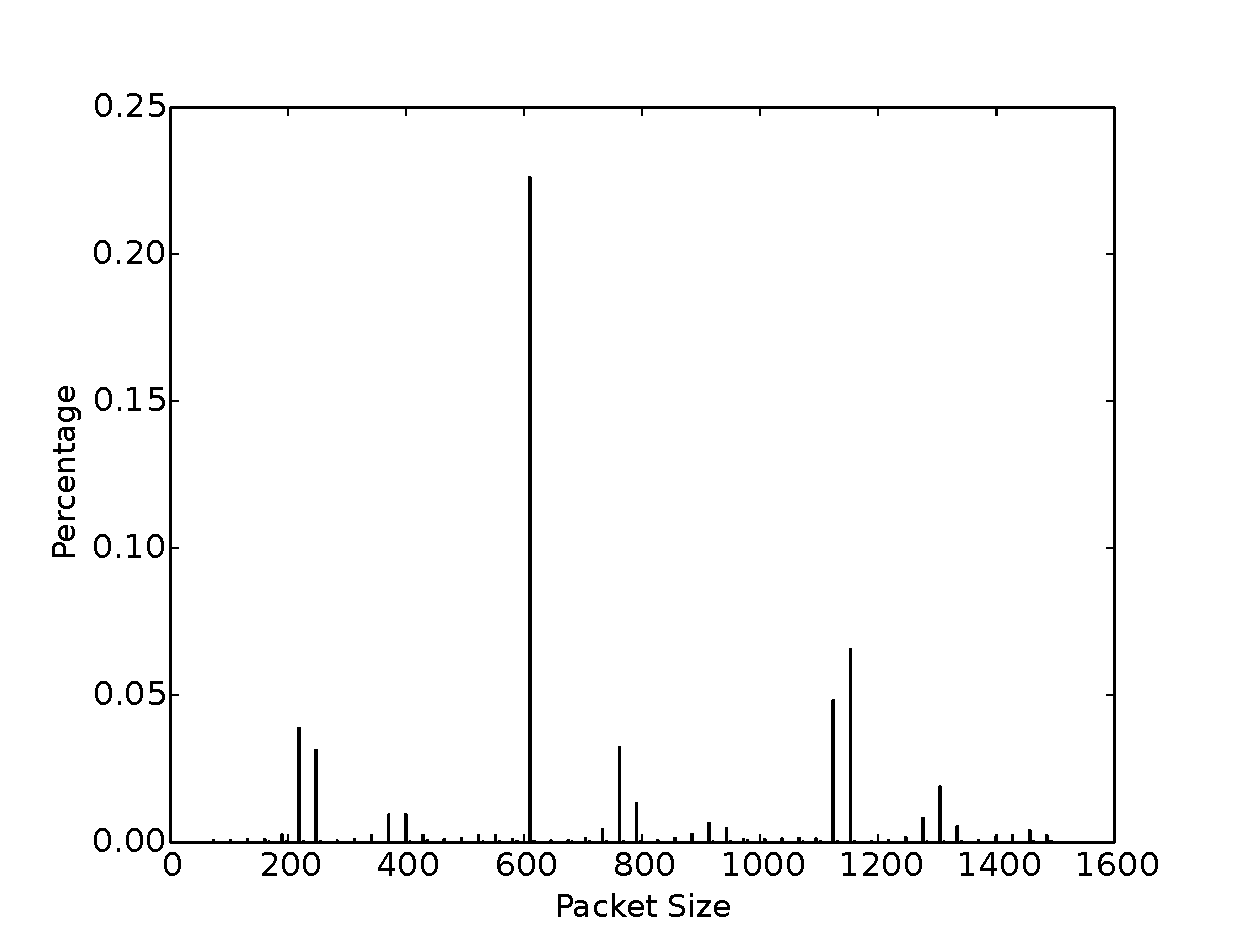
\includegraphics[width=\linewidth]{image/tor_reg_traffic_pkt_size_upstream.eps}
\caption{HTTP, upstream}
\label{fig:tor_reg_traffic_pkt_size_upstream}
\end{subfigure}
\begin{subfigure}{0.48\linewidth}
\centering
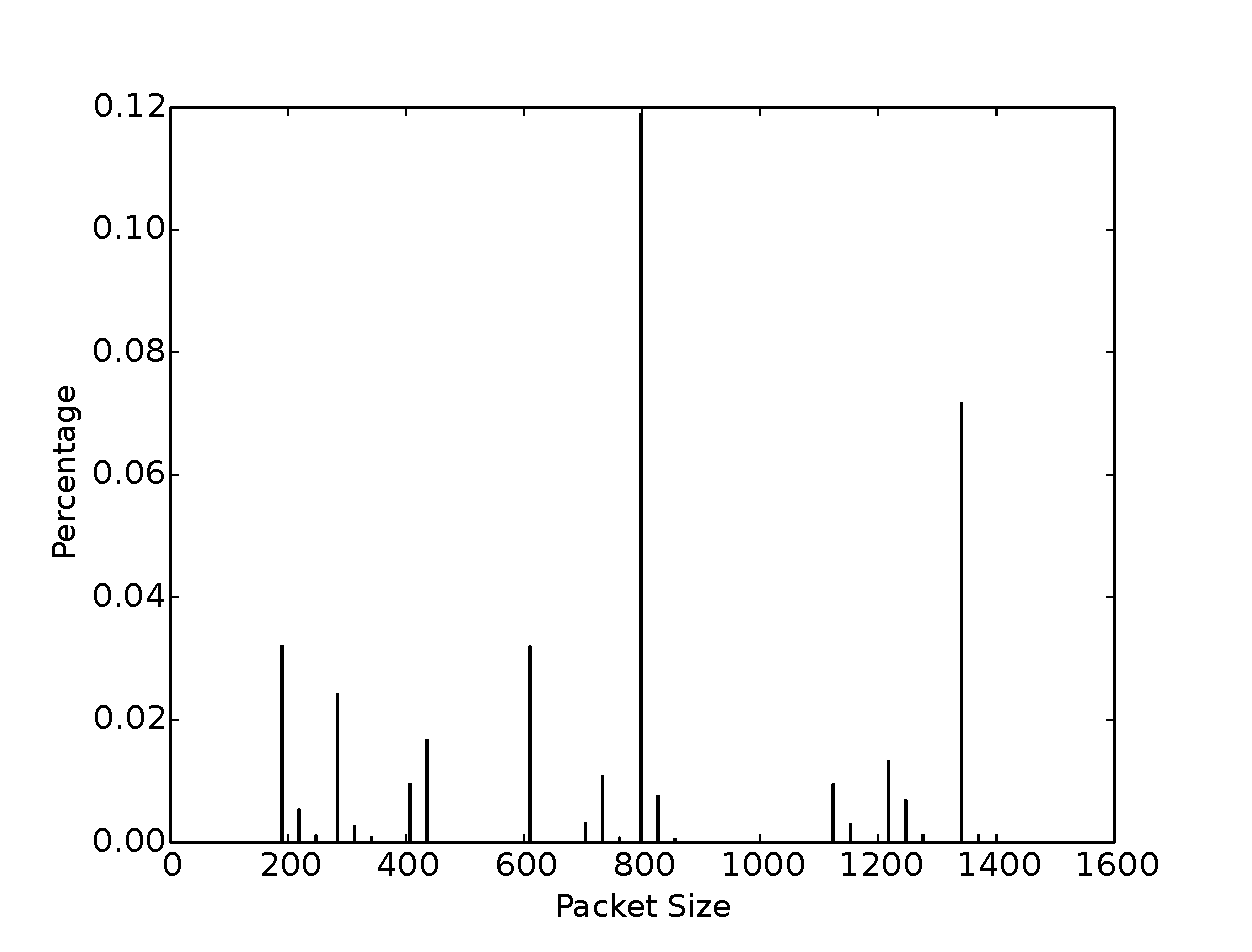
\includegraphics[width=\linewidth]{image/tor_reg_traffic_pkt_size_downstream.eps}
\caption{HTTP, downstream}
\label{fig:tor_reg_traffic_pkt_size_downstream}
\end{subfigure} 
\begin{subfigure}{0.48\linewidth}
\centering
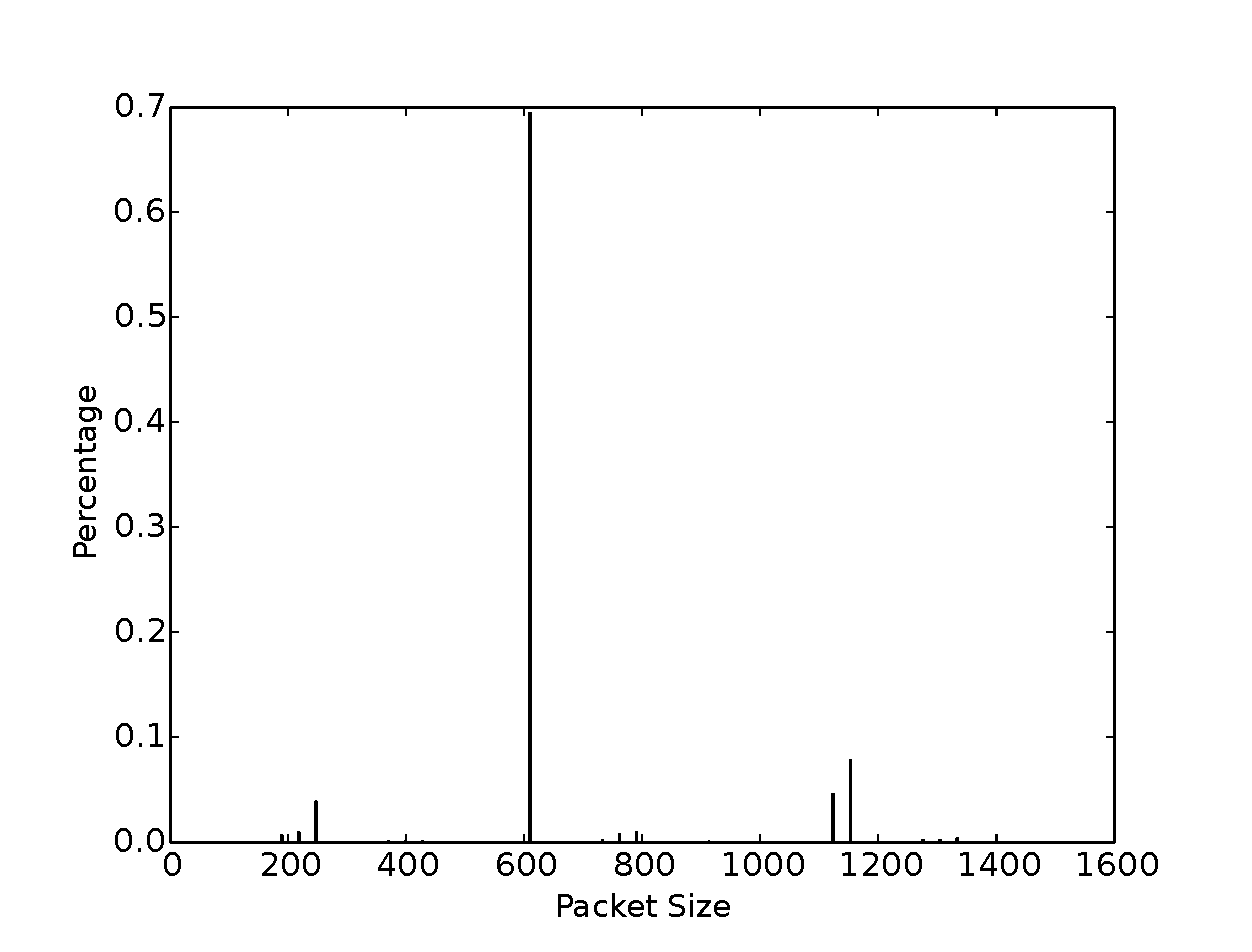
\includegraphics[width=\linewidth]{image/tor_compact_block_pkt_size_upstream.eps}
\caption{Bitcoin, Compact block, upstream}
\label{fig:tor_compact_block_pkt_size_upstream}
\end{subfigure}
\begin{subfigure}{0.48\linewidth}
\centering
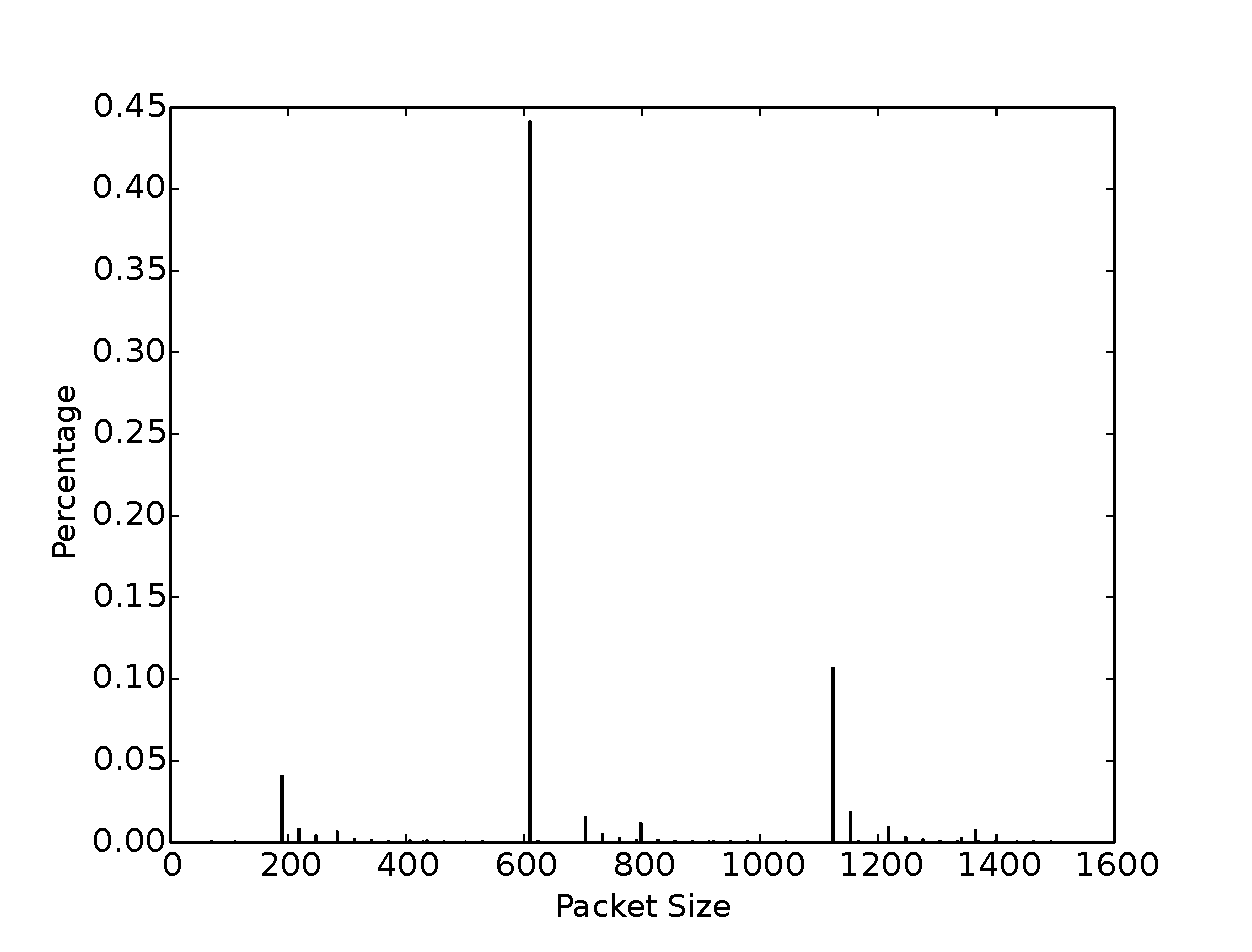
\includegraphics[width=\linewidth]{image/tor_compact_block_pkt_size_downstream.eps}
\caption{Bitcoin, Compact block, downstream}
\label{fig:tor_compact_block_pkt_size_downstream}
\end{subfigure} 
\begin{subfigure}{0.48\linewidth}
\centering
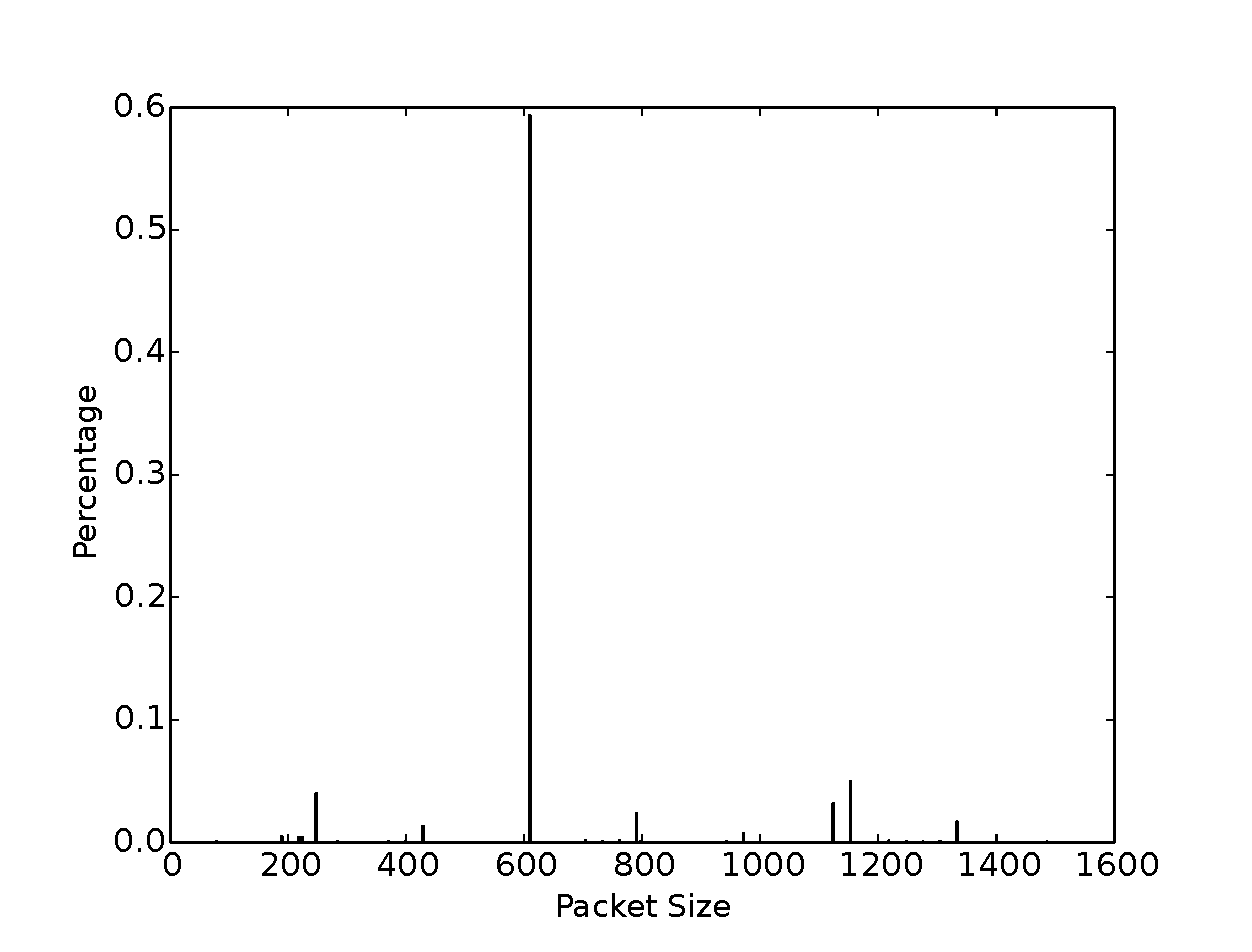
\includegraphics[width=\linewidth]{image/tor_fullblock_pkt_size_upstream.eps}
\caption{Bitcoin, Full block, upstream}
\label{fig:tor_fullblock_pkt_size_upstream}
\end{subfigure}
\begin{subfigure}{0.48\linewidth}
\centering
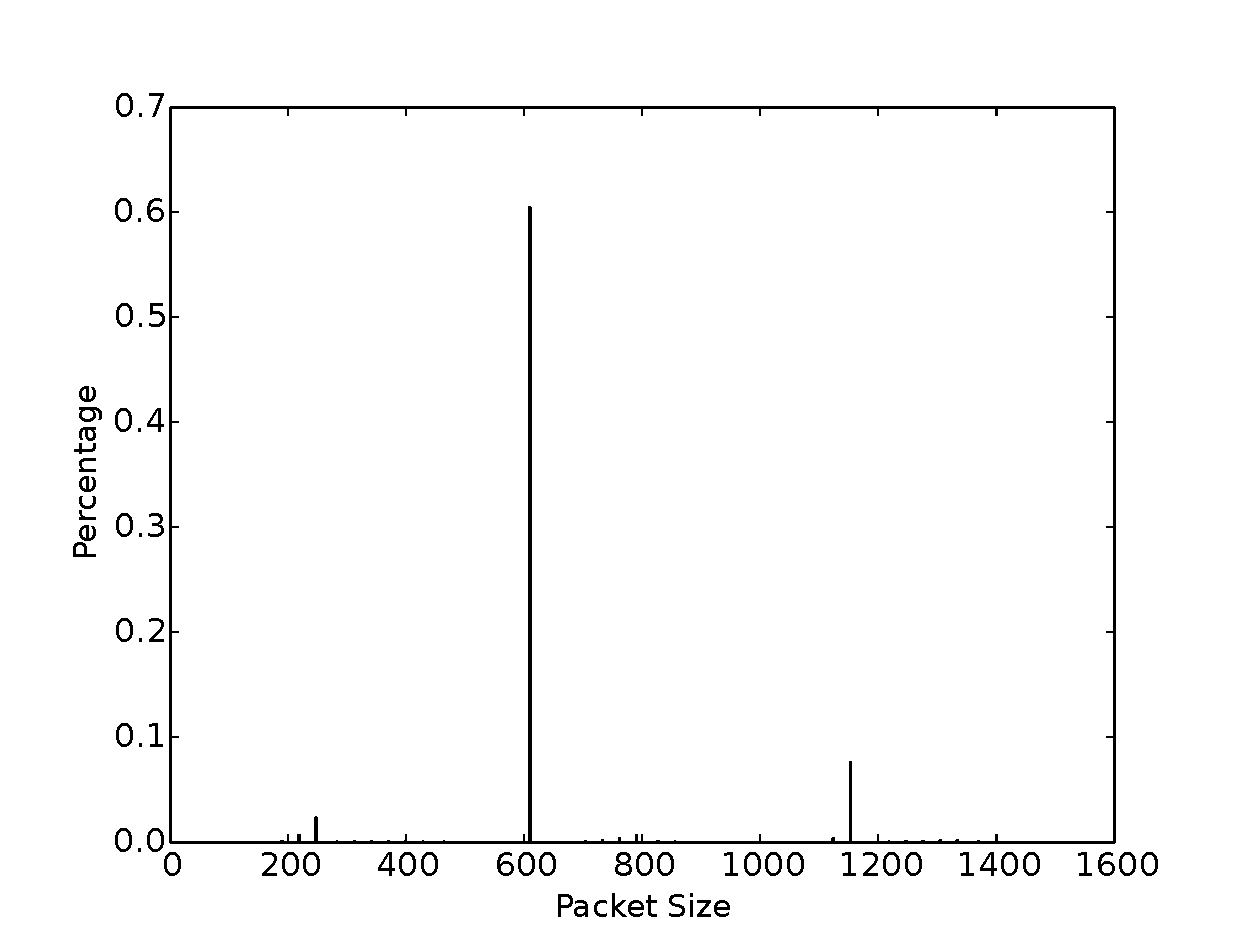
\includegraphics[width=\linewidth]{image/tor_fullblock_pkt_size_downstream.eps}
\caption{Bitcoin, Full block, downstream}
\label{fig:tor_fullblock_pkt_size_downstream}
\end{subfigure}
\caption{Distribution of packet sizes of HTTP and Bitcoin traffic behind Tor}
\end{figure}
\end{comment}
%\section{Algorithm for Window-based classifier}

\section{Threat Model}



\fatemeh{we did not have any text in here. }
\red{this section is so bad. it is not about threat model and it is too short. please put back the previous text that we had so i edit. }


 




